\subsection{Flat ground}
Over flat ground the map is the identity and the terrain-following propagator
reproduces \texttt{RationalHelmholtzPropagator}, including the NLBC, to
$4\cdot10^{-14}$ (unit test \texttt{TestFlatGroundEquivalence}).
\subsection{Exact solution: beam reflected by a perfectly conducting slope}\label{sec:slope}
The incident field is a complex-source-point beam at \SI{300}{MHz}, an exact
solution of the Helmholtz equation, with waist at $(-50,30)$\,m, Rayleigh parameter
\SI{100}{m} and direction $-10^\circ$. Its image in the line $z=x\tan\theta_s$ gives
the exact field above the Dirichlet slope. The reflected beam leaves at
$2\theta_s+10^\circ$, i.e.\ $30$, $50$ and $70^\circ$ for $\theta_s=10$, $20$ and $30^\circ$.
\begin{itemize}
\item Both solvers start from the exact field: on the curved trajectory $\xi=0$
(boundary not mirrored at $x=0$) and on the line $x=0$ respectively.
\item Both use Pad\'e $(7,8)$, the aperture $\theta_{\max}=10^\circ+2\theta_s+5^\circ$
and grids chosen by the respective optimizers.
\item The error is $\max|u-u_{\rm exact}|/\max|u_{\rm exact}|$ over the computational
domain above the ground.
\end{itemize}
\begin{table}[h]\centering
\caption{Exact slope test (Pad\'e $(7,8)$, precision parameter $10^{-2}$).}\label{tab:slope}
\begin{tabular}{rrrrrrrr}\toprule
& & \multicolumn{3}{c}{terrain-following} & \multicolumn{3}{c}{staircase}\\
\cmidrule(lr){3-5}\cmidrule(lr){6-8}
$\theta_s$ & aperture & $\Delta x$, m & $\Delta z$, m & error & $\Delta x$, m & $\Delta z$, m & error\\\midrule
$10^\circ$ & $35^\circ$ & 2.50 & 0.0345 & $1.4\cdot10^{-4}$ & 2.50 & 0.0625 & $5.4\cdot10^{-1}$\\
$20^\circ$ & $55^\circ$ & 2.50 & 0.0192 & $1.2\cdot10^{-3}$ & 2.50 & 0.0345 & $6.9\cdot10^{-1}$\\
$30^\circ$ & $75^\circ$ & 1.00 & 0.0093 & $2.9\cdot10^{-3}$ & 1.00 & 0.0159 & $8.1\cdot10^{-1}$\\
\bottomrule\end{tabular}\end{table}
\begin{figure}[t]\centering
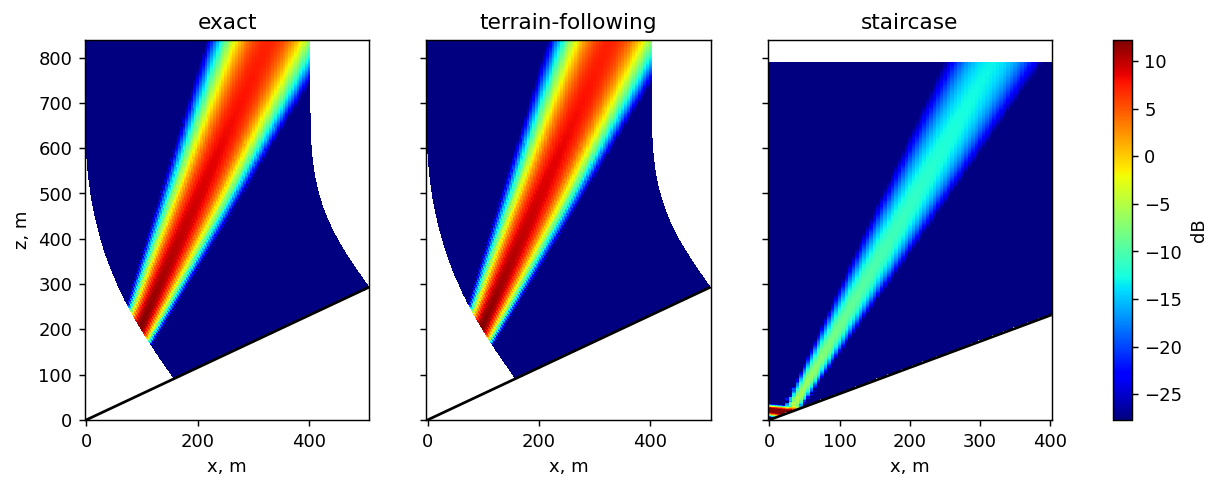
\includegraphics[width=\textwidth]{slope_exact_30deg_maps.png}\\
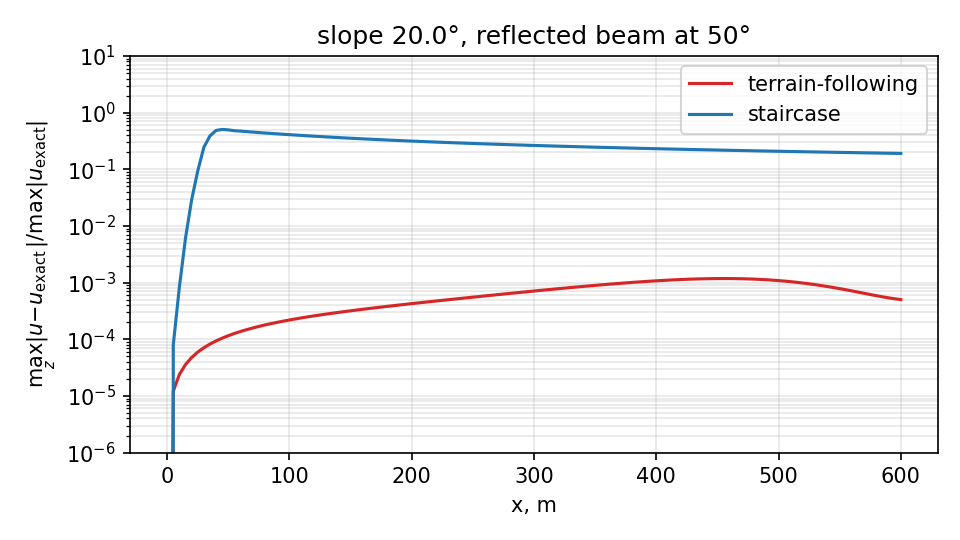
\includegraphics[width=0.49\textwidth]{slope_exact_20deg_error.png}\hfill
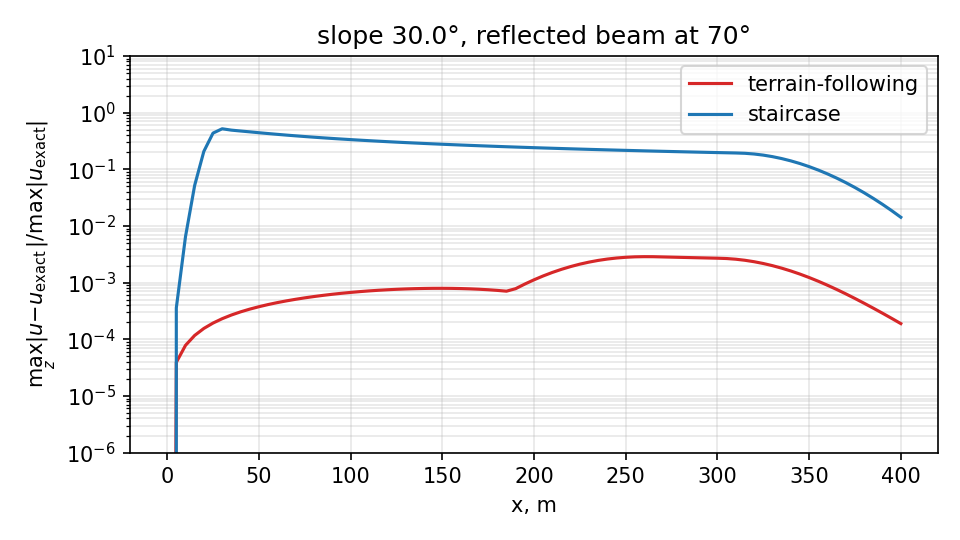
\includegraphics[width=0.49\textwidth]{slope_exact_30deg_error.png}
\caption{Beam reflected by a perfectly conducting slope. Top: $|u|$ for
$\theta_s=30^\circ$ (reflected beam at $70^\circ$); the terrain-following domain is
bounded by the curved trajectories $\xi=0$ and $\xi=x_{\max}$. Bottom: error versus
range for $\theta_s=20^\circ$ and $30^\circ$.}\label{fig:slope}
\end{figure}
The terrain-following error (\cref{tab:slope}, \cref{fig:slope}) is
$10^{-4}$--$3\cdot10^{-3}$ up to a reflected beam at $70^\circ$, on grids
comparable to those of the staircase. The staircase loses most of the reflected
beam, and its error is $0.5$--$0.8$. Refining the staircase grid for $\theta_s=20^\circ$ to
$\Delta z=0.005$\,m ($\lambda/200$) leaves the error at 0.54, and with
$\Delta x=0.625$\,m it is still 0.45: the staircase error is
geometric and decreases only slowly.

The flux-conserving step is essential:
\begin{itemize}
\item With the Liouville rescaling alone ($q=0$) the error in the $20^\circ$ case is
$6.4\cdot10^{-2}$, an amplitude drift along the reflected beam. Without the
rescaling it is larger still.
\item With unrotated $[2/2]$ factors a spurious evanescent component grows to
$0.14$ (\cref{sec:transformed}).
\item The rotated factors give $1.2\cdot10^{-3}$.
\end{itemize}
\subsection{Penetrable wedge}
The upslope wedge of the ASA benchmark \cite{jensen1990benchmark} has the
following parameters:
\begin{itemize}
\item \SI{25}{Hz}, water $c=\SI{1500}{m/s}$;
\item bottom \SI{1700}{m/s}, $\rho=1.5$, \SI{0.5}{dB/\lambda};
\item source at \SI{100}{m};
\item depth \SI{200}{m} with a flat lead-in to \SI{500}{m}, then a $2.86^\circ$ upslope to \SI{3.5}{km}.
\end{itemize}
All solvers use the same smoothed bathymetry ($\sigma=\SI{20}{m}$) and start from
the self-starter of RAM~1.5 at $r=\SI{1}{m}$; a patched copy of RAM writes it out.
RAM is single precision. On fine grids its tridiagonal systems lose all
accuracy: at $\Delta r=\SI{1}{m}$, $\Delta z=\SI{0.05}{m}$ the field is wrong by
\SI{77}{dB}. We therefore rebuilt it in double precision. It then converges: the
grids $(2.5,0.1)$\,m and $(1,0.025)$\,m differ by \SI{0.013}{dB} (median),
and the latter is the reference.
\begin{table}[h]\centering
\caption{Penetrable wedge: median / 90th percentile of $|\Delta\mathrm{TL}|$ (dB) with
respect to the RAM reference, $r>\SI{200}{m}$.}\label{tab:wedge}
\begin{tabular}{lcc}\toprule
solver (grid) & $z=\SI{30}{m}$ & $z=\SI{150}{m}$\\\midrule
terrain-following ($\Delta x=5$, $\Delta z=0.5$\,m) & 0.05 / 0.22 & 0.13 / 0.33\\
same scheme, stair-step bottom ($\Delta x=5$, $\Delta z=1.0$\,m) & 0.54 / 1.29 & 0.82 / 2.07\\
RAM ($\Delta r=10$, $\Delta z=0.5$\,m) & 1.66 / 6.70 & 2.79 / 10.42\\
\bottomrule\end{tabular}\end{table}
\begin{figure}[t]\centering
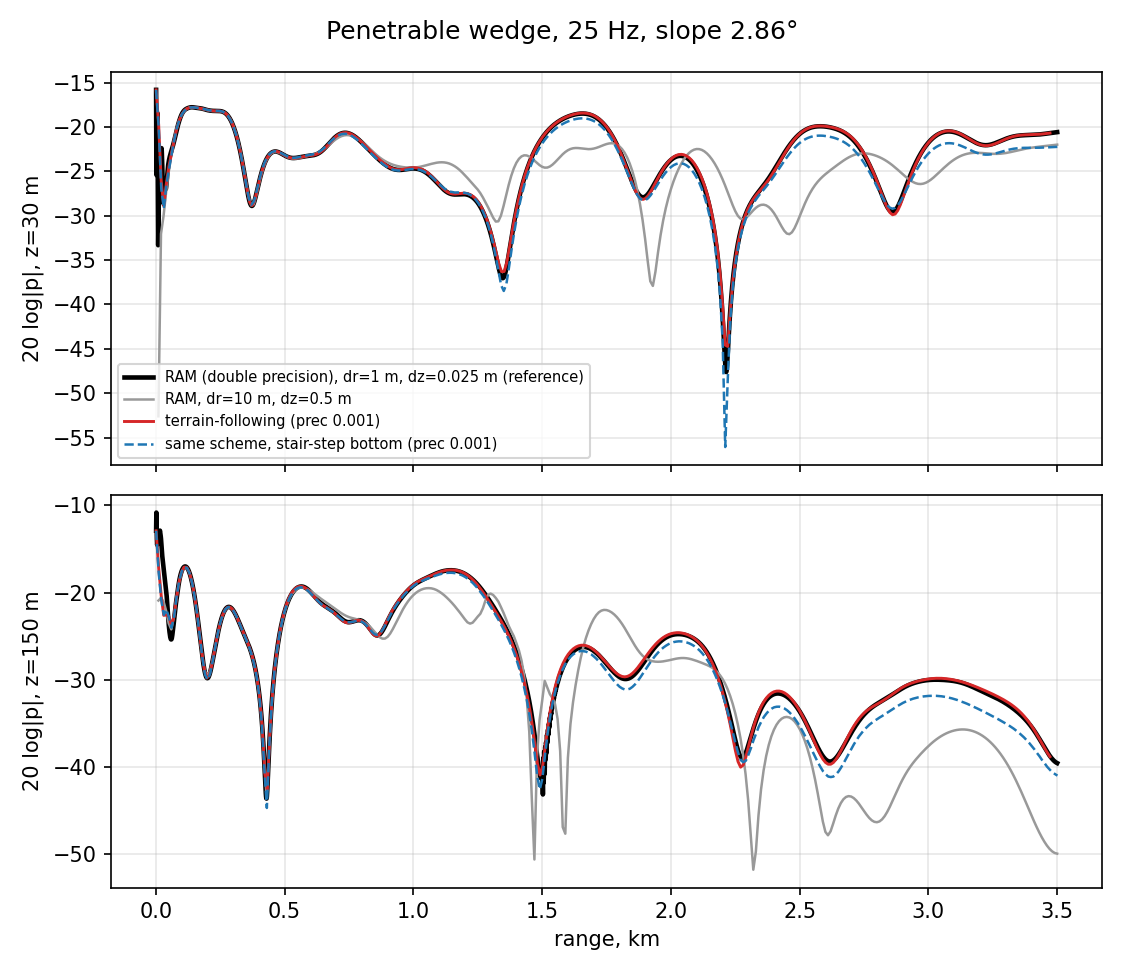
\includegraphics[width=0.66\textwidth]{wedge_uwa_25hz_cuts.png}\hfill
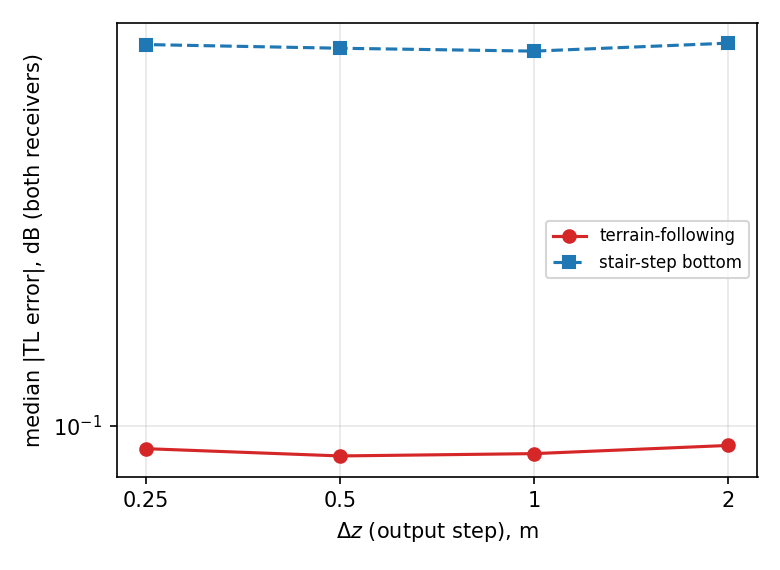
\includegraphics[width=0.33\textwidth]{wedge_uwa_25hz_convergence.png}
\caption{Penetrable wedge. Left: $20\log|p|$ at \SI{30}{m} and \SI{150}{m} depth.
Right: median error versus $\Delta z$ at the same range step.}\label{fig:wedge}
\end{figure}
The terrain-following solution agrees with the reference to
0.05--0.13\,dB (\cref{tab:wedge},
\cref{fig:wedge}). The stair-step bottom in the same scheme gives
0.5--0.8\,dB.

Refining $\Delta z$ from 2 to \SI{0.25}{m} does not reduce either error
(terrain-following 0.09--0.09\,dB, stair-step
0.68--0.71\,dB), and neither does refining
$\Delta x$ to \SI{1.25}{m} or raising the flux order to $q=3$. The two floors have
different origins:
\begin{itemize}
\item \emph{Stair-step.} This is the energy-conservation defect of one-way models
across vertical density steps \cite{porter1991energy}. Each step makes an error
$O(\Delta h)$ and there are $O(1/\Delta h)$ steps, so the bias does not vanish.
RAM avoids it through its density-scaled variable.
\item \emph{Terrain-following.} The residual of about \SI{0.1}{dB} is the
difference between two one-way models of the same sloping interface (RAM's
stair-steps, ours continuous). It is grid-independent. It is larger at the
receiver that lies in the sediment beyond \SI{1.5}{km}.
\end{itemize}
